%!TEX root = main.tex
%\comment[id=SDIV]{Fix this section.}
We use an extension of the classical Kermack-McKendrick model.
Our formulation considers vaccination and vital dynamics. To this end, for fixed time $t$, we 
split the total population $N(t)$, according to the following compartments: 
susceptible ($S(t)$), 
exposed ($E(t)$),
symptomatic infectious ($I_S(t)$),
asymptomatic infectious ($I_A(t)$),
recovered ($R(t)$), 
dead ($D(t)$) and vaccinated ($V(t)$).
Our formulation requires the following hypotheses: 
\begin{enumerate}[(\textbf{H}-1)]
    \item
        The vaccine is administered to all individuals
        exempting those with symptoms. Therefore, only individuals in the $S$, $E$, $I_A$ and $R$ 
        classes are candidates for vaccination. 
    \item    
        The vaccine only has effects on the susceptible individuals. Thus, 
        susceptible individuals become vaccinated at $\psi_V$ rate.
    \item 
        The vaccine only protects against COVID-19.
    \item
        Individuals get vaccinated only once during the epidemic. 
    \item Once an inoculated individual gets vaccine-induced immunity, returns to the
    $S$ class after a period of time (waning immunity period).
    \item 
        The vaccine is imperfect. A fraction
        of individuals in $V$ may become infected, with a lower 
        probability than those in the $S$ class. 
    \item After a natural immunity period, the recovered population returns to the 
    susceptible class. 
\end{enumerate}

    Since we will explore disease dynamics that lasts from six months to one year, 
the model includes vital dynamics. We consider a constant population $(N(t)= N)$. Thus, we assume that birth and 
natural death rates are the same
and represented by $ \mu $. All births lie into the $S$ class and all but class $D$ experience 
natural death. Class $D$ does not intervene in the transmission
dynamics and counts reported deaths. 

    The infection dynamics are as follows: Susceptible individuals $(S)$ become 
infected, but not infectious, when in contact with infectious
individuals $I_S$ and $I_A$. Exposed individuals ($E$) remain in their class until they become
infectious and move to either $I_S$ or $I_A$. Individuals in class $I_S$ either die by disease
complications or recover, whereas individuals in class $I_A$ move to the $R$ class after a some time. Finally, as the vaccine is considered imperfect, individuals in $V$ move to the $E$ class
by interacting with infectious individuals $I_S$ and $I_A$ at a lower rate than $S$ individuals. 
\Cref{Fig:SchemeModel} shows the compartmental model diagram which summarizes hypotheses mentioned above.

\begin{figure*}[tbh]
    \centering
    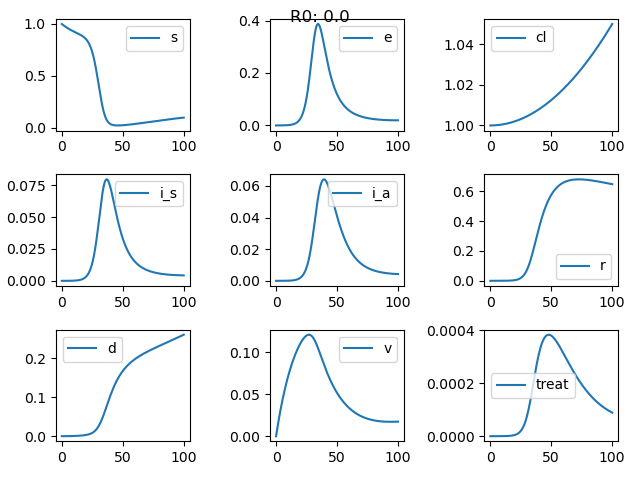
\includegraphics[scale = 1]{Figure_1.pdf}
    \caption{%
        Compartmental diagram of COVID-19 transmission dynamics which 
        including vaccination dynamics. Here, there are seven different classes: 
        Susceptible $(S)$, exposed $(E)$, symptomatic infected $(I_S)$, asymptomatic 
        infected $(I_A)$, recovered $(R)$, death $(D)$ and vaccinated $(V)$ 
        individuals.}
    \label{Fig:SchemeModel}
\end{figure*}
%
The model is given by the following ordinary differential equations system
%
\begin{equation}\label{model1}
    \begin{aligned}
        S'(t) &= \mu \widehat{N}-f_{\lambda} S - (\mu+\psi_V)S +
        \omega_V V+ \sigma_R R
        \\
        E'(t) &= f_{\lambda}\left(S+
        (1-\varepsilon_V) V\right)-(\mu+\sigma_E) E 
        \\
        I'_S(t) &= 
        p \sigma_E E-(\mu+\alpha_S) I_S
        \\
        I'_A(t) &= (1-p) \sigma_E E-(\mu+\alpha_A) I_A 
        \\
        R'(t)&= (1-\theta) \alpha_S I_S +
        \alpha_A I_A-(\mu+\sigma_R) R 
        \\
        D'(t) &= \theta \alpha_S I_S 
        \\
        V'(t) &= \psi_V S-(1-\varepsilon_V)  
        f_{\lambda}V - (\mu+\omega_V) V
        \\
    \end{aligned}
\end{equation}

where the infection force is defined by
\begin{equation}\label{infection-force}
    f_{\lambda}:=\frac{\beta_S I_S + \beta_AI_A}{\widehat{N}}.
\end{equation}
%
Here, $\widehat{N}(t)=S(t)+E(t)+I_S(t)+I_A(t)+R(t)+V(t)$. For system in
\Cref{model1} all the
variables are taken normalized by the constant total population $N$. Therefore
$\widehat{N}+D = 1$.

Let
$$
    \Omega=
        \{
            (S,E,I_S,I_A,R,D,V) \in [0,1]^{7}: 
            S+E+I_S+I_A+R+D+V=1
        \} \subset [0,1]^{7}.
$$

The dynamics in \Cref{model1} is positively-invariant on $\Omega$ 
(see \Cref{apx:positivity_invariace}). Additionally, the equations
\begin{equation}
    \label{eqn:model1_counters}
    \begin{aligned}
        X'(t) &=
        \psi_V(S + E + I_A + R)
        \\
        Y'_{I_S}(t) &=p
        \sigma_E E,
    \end{aligned}
\end{equation}
%
count the cumulative administered vaccines doses until time $t$ as the product 
$N\times X(t)$.
Also, the cumulative incidence of reported cases is given by 
$N\times Y_{I_S}(t)$.
\begin{rmk}
    Vaccine is administered to individuals in classes $S$, $E$, $I_A$ and $R$. 
    The amount of given vaccines is quantified by \Cref{eqn:model1_counters}. 
    However, as we 
    assume the vaccine has preventive nature only, there is no change from 
    classes $E$, $I_A$, and 
    $R$ to $V$ due to vaccination. 
\end{rmk}

The parameters of model \Cref{model1} are described in 
\Cref{table:parametermodel}.
\begin{table*}[tbh]
    \centering
    \begin{tabular}{
        >{\centering}
        p{0.2\textwidth}
        p{0.6\textwidth}
    }
        \toprule
        Parameter & Description
        \\
        \midrule
        $\mu$ &  Natural death rate
        \\
        $\beta_S\ (\beta_A)$ & 
            Symptomatic (Asymptomatic) transmission contact rate
        \\
        $\psi_V$ & Vaccination rate
        \\
        $\omega_{V}$ & 
            Waning rate of vaccine. 
            $1/\omega_{V}$ is the average time to lose vaccine-induced immunity
        \\
        $\varepsilon_V$ &  Vaccine efficacy
        \\
        $\sigma_{E}$ & 
        Latency rate. $1/\sigma_{E}$ 
                is the average latency period
        \\
        $p$ & 
            Exposed individuals' fraction who become symptomatic infectious
        \\          
        $\alpha_{S}$ &
            Transition rate from symptomatic to recover or death. 
            $1/\alpha_{S}$ is the average output time of symptomatic individuals class
        \\
        $\theta$ & 
            Proportion of symptomatic individuals who die due to 
            the disease 
        \\ 
        $\alpha_{A}$ 
            & 
            Recovery rate of asymptomatic individuals. $1/\alpha_{A}$ is the
            average time which asymptomatic individuals 
            leave being infectious 
        \\ 
        $\sigma_{R}$ 
            &  
            Rate of loss of natural immunity.  
            $1/\sigma_{R}$ is the natural immunity period
        \\
        \bottomrule
    \end{tabular}
    \caption{Parameters definition of system in \Cref{model1}.}
    \label{table:parametermodel}
\end{table*}
%
\subsection{Calibration of baseline parameters and initial conditions}
%\added[id=MAAZ, comment=AR 1.3 2.6]{
    Multiple COVID-19 studies %\cite{Acuna2020, Barbarossa2020, Sardar2020} 
have shown important differences in transmission contact rates values across 
countries. For this reason, we establish a set of baseline parameter values 
for our geographic region of interest: the area constituted by Mexico-City 
and Mexico-State.

    Mexico’s COVID-19 database provides detailed information on reported 
cases, hospitalized,
ambulatory and deaths. Following the ideas of \az [Fergunson]\za, we consider 
COVID-19 confirmed deaths data to calibrate both transmission contact rates and exposed individuals proportion who become symptomatic infectious.

    To address this problem, we employ a MCMC method. As observation model, we use a negative
binomial distribution with mean given by
\begin{equation}\label{incidence}
    \begin{aligned}
        \widehat{D}(k) = D(k) - D(k-1)=\int_{k-1}^k \theta\alpha_{S}I_{S}(t) dt,
    \end{aligned}
\end{equation}
where $\widehat{D}(k)$ represents the daily deaths incidence at the $k-th$ day,
and $D(k)$ is the solution of the sixth equation of the system in \Cref{model1}
without vaccination dynamics at the $k-th$ day. \Cref{Fig:fittingcurve} shows 
fitting curves with their respective confidence bands.
Estimation process considers data from February 19, 2020, to October 31, 2020. 
Like other studies \cite{Acuna2020,Santana2020}, it is considered 
perturbations on both transmission contact rates due to implementing or 
breaking mitigation measures. 
For more information about the parameter estimation process, 
see \Cref{App:Parameter_Est}. \Cref{table_icparam} 
summarizes our parameter calibration.
%
\begin{table}[tbh]
    \begin{center}
        \begin{tabular}{lll}
            \toprule
            Parameter & Estimated range & Calibrated
            \\
            \midrule
            $\beta_S$ & $[\num{0.058262},\  \num{0.544492}]$ & $0.363282$ 
            \\
            $\beta_A$ & $[\num{0.101754},\ \num{0.441215}]$ & $0.251 521$ 
            \\
            $p$       & $[\num{0.111348},\ \num{0.249985}]$ & $0.1213$ 
            \\
            \bottomrule
        \end{tabular}
        \caption{%
            Estimated range for some parameters of system in \Cref{model1}
        without vaccination dynamics.
        }\label{table_icparam}
    \end{center}
\end{table}
%
\begin{figure*}[tbh]
\centering
    \includegraphics[scale=1]{Figure_2.png}
    \caption{
        \az Fitting death curve of the COVID-19 outbreak 
        in Mexico-City and Mexico-State. \za
        Panel A shows new reported deaths per day. 
        Panel B represents cumulative deaths per day.
        Reported deaths data are shown in blue bars from February 19,
        2020, to October 31, 2020.
    }
    \label{Fig:fittingcurve}
\end{figure*}
\begin{figure*}[tbh]
\centering
    \includegraphics[scale=1]{Figure_2_1.png}
    \caption{
        \az Fitting death curve of the COVID-19 outbreak 
        in Mexico-City and Mexico-State. \za
        Panel A shows new reported deaths per day. 
        Panel B represents cumulative deaths per day.
        Reported deaths data are shown in blue dots from February 19,
        2020, to October 31, 2020.
    }
    \label{Fig:fittingcurve}
\end{figure*}
